\chapter{Grundlagen der Plugin Entwicklung}
\label{cha:Grundlagen}

\section{Entwicklungsumgebungen}
\label{sec:Entwicklungsumgebungen}

\subsection{Visual Studio Code}

\subsection{IntelliJ IDEA}


\section{Programmiersprachen}
\label{sec:Programmiersprachen}

\subsection{TypeScript}

Die TypeScript Programmiersprache wurde erstmalig am 1. Oktober 2012 [17] von 
Microsoft in Form eines open-source Projekts veröffentlicht. Designed wurde sie 
von Anders Hejlsberg, der auch an der Entwicklung von C\# beteiligt war. 

Die grundsätzliche Idee der Sprache ist, eine typsichere, kompilierte, und somit 
bessere Version von JavaScript zu sein. JavaScript ist aufgrund des Erfolgszugs
des Internets zu einer sehr wichtigen Sprache geworden und war auch schon 2012 
aus den TOP Listen für Programmiersprachen nicht mehr wegzudenken [8][21] [22]. 
Webseiten setzen heute sehr stark auf JavaScript, um durch interaktive Elemente 
die User Experience zu verbessern oder um neue Funktionalität anbieten zu können. 
Durch das Node.js runtime environment kann JavaScript nicht mehr nur im Browser 
verwendet werden, sondern es können auch Desktop, Server oder Mobile Anwendungen 
in JavaScript entwickelt werden. Durch diesen großen Umfang an Möglichkeiten die 
JavaScript dadurch bietet werden natürlich auch immer größere Projekte damit entwickelt. 
Und hier kommen die großen Schwächen von JavaScript immer mehr zu tragen. 
Je größer die Projekte werden und je mehr EntwicklerInnen an einem Projekt 
mitarbeiten, desto mehr Fehler entstehen aufgrund der fehlenden Typsicherheit
und des fehlenden Compilerschrittes. Diese Schwachstellen versucht TypeScript 
nun auszubessern.

TypeScript code wird mithilfe des TypeScript Compilers „tsc“ in einfache JavaScript 
Dateien transpiliert. Dadurch kann auf die Popularität und Verbreitung von JavaScript 
aufgebaut werden und TypeScript ist überall dort verwendbar, wo JavaScript 
ausführbar ist. Weiters ist TypeScript ist ein Superset von JavaScript. 
Es gilt also: „Any valid .js file can be renamed .ts and be compiled with other 
TypeScript file.” [23]. 

Jedoch bietet TypeScript eine Menge von Vorteilen 
gegenüber ihrer Basissprache.
\begin{itemize}
  \item Durch den Kompilierschritt mit dem tsc Compiler wird der Code vor der Ausführung automatisch auf Validität geprüft. Es entfällt also die Notwendigkeit für einen zusätzliches Linting Tool wie JSLint. Dieser Compile-Schritt kann natürlich auch in eine CI/CD Pipeline eingebunden werden, um auch bei Merges Feedback über die Validität des Codes zu erhalten.
  \item Durch die statische Typisierung können Missverständnisse über die Verwendung von Variablen vermieden werden. Auch die Unterstützung durch verschiedene IDEs, zum Beispiel mittels IntelliSense kann durch die Typen verbessert werden. Dies ist nicht nur bei der Zusammenarbeit hilfreich, sondern kann auch die Arbeit jeder einzelnen EntwicklerIn beschleunigen.
  \item In TypeScript können Klassen erstellt werden, deren Properties mit Zugriffsmodifikatoren (private/public) versehen sind.
  \item TypeScript unterstützt Vererbung, Interfaces und generische Programmierung.
  \item In TypeScript können bereits bestehende JavaScript Bibliotheken wiederverwendet werden. Weiters ist es möglich durch zusätzliche Dateien Typinformationen zu den bestehenden Bibliotheken zu liefern.
\end{itemize}

\subsection{Java}

Die Entwicklung der Programmiersprache Java begann im Jahr 1991 und sie 
wurde von den James Gosling, Mike Sheridan und Patrick Naughton designed. 
[24] Java wurde erstmals im Jahr 1995 von Sun Microsystems veröffentlicht. 
Im Januar 2010 wurde Sun Microsystems dann von der Oracle Corporation übernommen, 
welche seitdem auch Java weiterentwickelt.

Das Design und vor Allem die Syntax der Sprache war stark von C und C++ inspiriert, 
um anderen Entwicklern einen leichten Umstieg auf das neue Java zu ermöglichen. 
Allerdings versuchte Java die teils sehr komplexen (wenn auch effektiven) 
Sprachfeatures von C++ etwas zu vereinfachen. Java sollte eine simple, objektorientierte 
und robuste Sprache werden. Die Funktionalität die Java zu dem großen Erfolg verhalf, 
den sie später hatte, war das „write once, run anywhere“ (WORA) Prinzip. Im Gegensatz 
zu den zuvor gängigen Programmiersprachen muss Java nämlich für bestimmte 
Hardwarearchitekturen kompiliert werden. Java Programme werden zu einer Art 
Zwischensprache, dem sogenannten Java Bytecode kompiliert. Dieser Bytecode
kann dann von einer Java Virtual Machine (JVM) ausgeführt werden. Diese JVM ist
im Grunde ein eigenständiges Programm welche mit dem Java Runtime Environment 
(JRE) mitgeliefert wird. Ein einmal kompiliertes Java Programm kann also auf 
allen Geräten ausgeführt werden, auf denen ein passendes JRE installiert ist. 
So ist es zum Beispiel auch möglich Java für die Entwicklung von Android nativen
Apps auf Mobilgeräten zu benutzen.

Ein weiterer Vorteil gegenüber älteren Sprachen wie C++ ist die
automatisierte Speicherverwaltung. Diese funktioniert mithilfe eines 
sogenannten „garbage collectors“ welcher nicht mehr benötigten Speicher
am Heap bereinigt und freigibt. Man kann also beliebig neue Objekte im Speicher
allokieren und muss sich nicht um die deallokierung der zuvor erstellten Objekte
kümmern. Auf diese Weise können häufige Programmierfehler wie Memory Leaks fast 
vollständig unterbunden werden.

Java unterstützt sowohl das objektorientierte, das prozedurale als auch das funktionale 
Programmierparadigma. Der Fokus liegt allerdings stark auf der Objektorientierung. 
Dabei bietet Java Funktionalitäten zur Abstraktion durch Verwendung von Klassen, Information Hiding
mithilfe von Zugriffsmodifikatoren (public/private/protected/package), Vererbung, 
Interfaces, Polymorphismus, Überladen von Methoden, generischer Programmierung, 
Exception Handling und vieles mehr.

\section{Aufbau der Plugin API}
\label{sec:AufbauDerPluginAPI}

\subsection{Visual Studio Code}

\subsection{IntelliJ IDEA}


\section{Funktionalität der Plugin API}
\label{sec:FunktionalitätDerPluginAPI}

\subsection{Visual Studio Code}

\subsection{IntelliJ IDEA}

\subsection{IntelliJ Flora Plugins}

In der Plugin Dokumentation von JetBrains wird zu Beginn 
empfohlen sich noch einmal gründlich zu überlegen, ob man 
für die von einem gewünschte Funktionalität wirklich ein 
vollwertiges Plugin benötigt. Häufig kommt es nämlich vor, 
dass nur bestimmte kleine Tasks innerhalb des IDEs 
automatisiert werden sollen. Hierfür schlägt JetBrains 
einige leichtgewichtige Alternativen vor. Eine nennenswerte 
Alternative ist das „Flora Plugin“ für das IntelliJ IDEA. 

Flora kann über die Einstellungen des IntelliJ IDEA 
im Abschnitt „Plugins“ installiert werden.

% //TODO rework screenshots

\begin{figure}
    \centering
    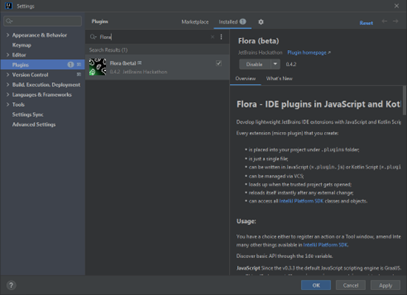
\includegraphics[width=.95\textwidth]{flora_plugin}
    \caption{Flora Plugin im IntelliJ Plugin Marketplace.}
    \label{fig:FloraPlugin}
\end{figure}    
 
Das Plugin sucht dann in den geöffneten Projektverzeichnissen
nach ausführbaren JavaScript oder Kotlin Script „micro plugin“ 
Dateien. Diese müssen sich in einem Ordner namens „.plugins“ 
befinden und auf „.plugin.js“ oder „.plugin.kts“ enden.
Innerhalb diese Plugin Dateien kann über die Variable „ide“ auf 
die angebotene Schnittstelle zugegriffen werden. Diese erlaubt 
es unter anderem Actions, Keyboard Shortcuts, Services und 
ToolWindows zu erstellen.

\begin{figure}
    \centering
    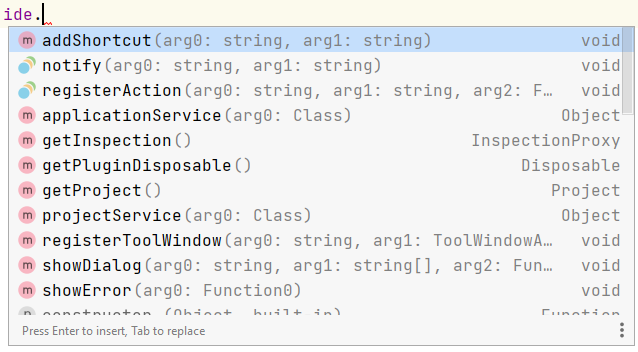
\includegraphics[width=.95\textwidth]{flora_codeCompletion}
    \caption{Übersicht über die API des Flora Plugins.}
    \label{fig:FloraPluginAPI}
\end{figure}    
 
Flora Plugins bieten sich vor allem dann an, wenn eine projektspezifische 
Aufgabe automatisiert werden soll. Hier sind vor Allem die 
Leichtgewichtigkeit der Plugins und die Schnelle, mit der ein 
einfaches Plugin entwickelt werden kann, von großem Vorteil. 
Weiters spricht für diesen Anwendungsfall, dass der Plugin Code 
direkt im Projektordner abgelegt wird und somit auch in einem Version 
Control System wie Git mit abgelegt werden kann.
